\chapter{Benchmarking Evolutionary Reinforcement Learning}
% BERL.jl for RL benchmarking}
\label{chap:berl}

\addlink{https://github.com/d9w/BERL.jl}{\berl}, short for \textit{Benchmarking Evolutionary Reinforcement Learning}, is a benchmarking tool created by my supervisor Dennis Wilson to compare the performance of Evolutionary Reinforcement Learning algorithms on a set of standard Reinforcement Learning benchmark tasks, for which I developed the architecture. 

\section{Motivation and structure}

% DGW: motivation ?

Even though benchmarks exist for Evolutionary Algorithms, such as \addlink{https://coco.gforge.inria.fr/}{COCO (COmparing Continuous Optimisers)}, they do not include Evolutionary RL algorithms, and focus on optimization of static problems which would be represented by the white rows in figure \ref{fig:GP-classes}. 

While comparisons of multiple RL algorithms are often provided in works such as \cite{CGP} defining new methods, they rely on values taken from other publications on the same standard environments, but in potentially different settings. Language speed and actual computational cost may not be the same in every case, introducing bias in the comparison and making it harder to know what algorithm is better.\\
Non-open-source code, such as OpenAI's algorithms for \dota, also raises the question of how to compare algorithms on an equal footing, and implementations adding features that were not included in the initial paper, like NEAT, make it harder to compare the performance of the algorithm behind.

Finally, benchmarking these algorithms is a technical challenge since implementations and environments can vary in languages, from Python to C++, and may also be implemented in deprecated versions of these languages.

Hence, as the Evolutionary RL and Genetic Programming fields need better benchmarks \cite{GP-benchmark} to compare algorithms on standardized tests, \berl aims to bring a versatile framework that allows this comparison and can be incrementally completed as new methods appear.

The code of \berl is voluntarily modular to allow adding more environments and new algorithms to the comparison. Hence, it relies on 3 blocks: algorithm \addlink{https://github.com/d9w/BERL.jl/blob/master/src/algorithms/CGP/_setup.jl}{\code{\_setup} files}, \addlink{https://github.com/d9w/BERL.jl/blob/master/src/environments/BERL_env.jl}{\code{BERLenv} structures}, and \addlink{https://github.com/d9w/BERL.jl/blob/master/src/core.jl}{the \code{start\_berl} method} to link them.
% DGW: individual BERL code links not necessary 

% DGW: image here? / DONE

\begin{figure}[H]
 \centering
 \captionsetup{justification=centering, margin=0.5cm}
 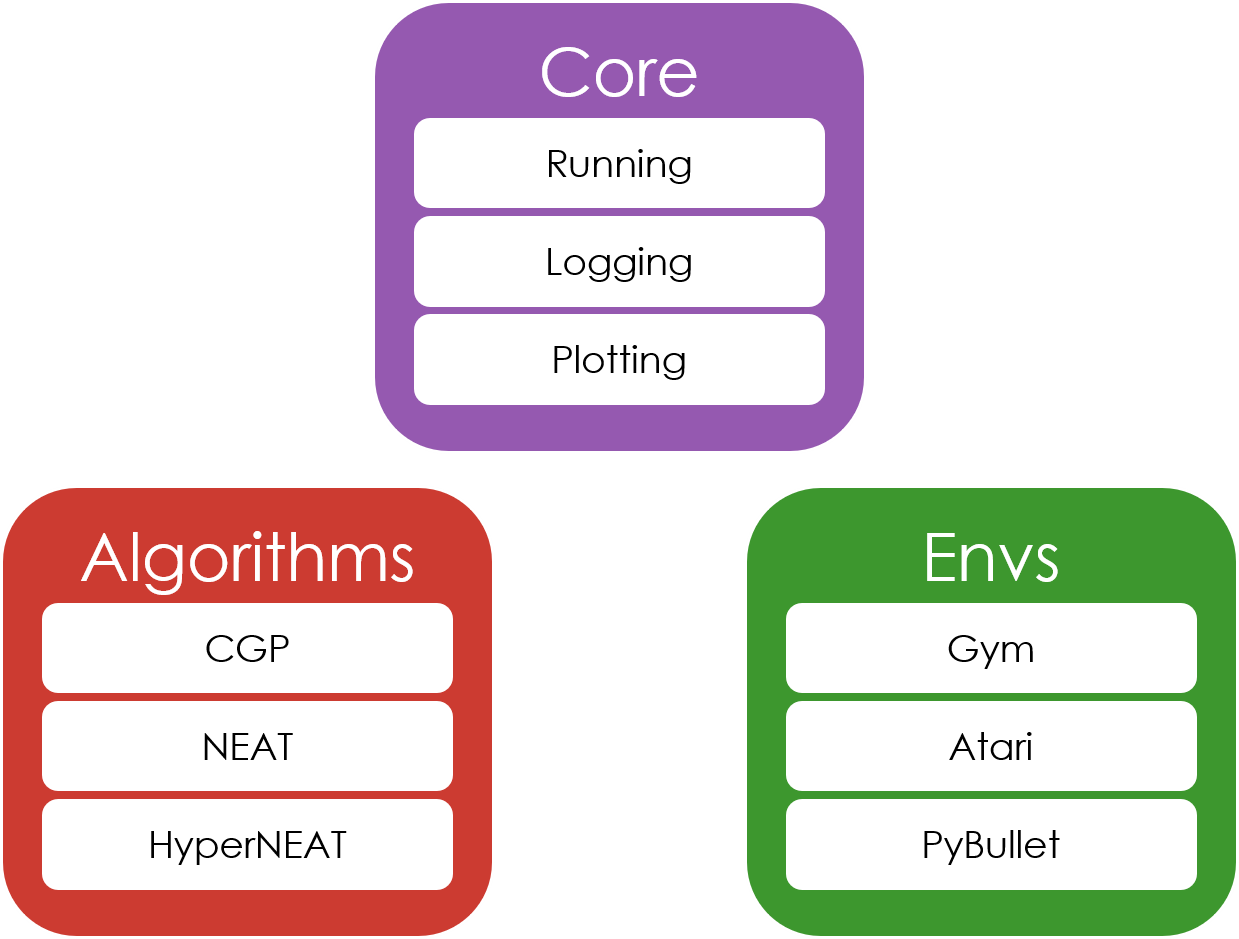
\includegraphics[height=8cm]{images/berl_archi.png}
\caption{Architecture of \berl in 3 blocks.}
 \label{fig:time-diff}
\end{figure}

\subsection{\code{\_setup} files}

Each algorithm requires a \code{\_setup} Julia file that includes a function returning a \\\code{Cambrian.Evolution} object from a configuration dictionary and a fitness function, and a \code{process} function to evaluate the algorithm with a specific input. This allows to use all algorithms the same way in the rest of the code through an algorithm-agnostic interface. 

Additionally, each algorithm has multiple \addlink{https://github.com/d9w/BERL.jl/blob/master/src/algorithms/CGP/gym.yaml}{YAML files}, each defining the run parameters for an environment. The \code{\_setup} and YAML files are all stored in the same folder named after the algorithm.

YAML files are used in this project for their compatibility with all languages, their simplicity of use, and their simplicity to read and write even for researchers not used to Julia. 

%DGW: Give example YAML file. Motivation for YAML: simplicity, easy to read and write

\subsection{\code{BERLenv} structure}

In order to also present a homogeneous interface on the environments side, the \addlink{https://github.com/d9w/BERL.jl/blob/master/src/environments/BERL_env.jl}{\code{BERLenv}} abstract type is used to wrap each environment and make them all interact with the same functions. For each benchmark, a \code{mutable struct} is created with all required elements inside, and the function building it is in charge of starting the simulator and setting the parameters.

The \code{fitness} method takes a \code{Cambrian.Individual} and evaluates it, returning its fitness in this environment. Finally, the \code{new\_gen} method can be used to reset the environment between generations or to give it a new random seed, making it stochastic between generations but deterministic for all evaluations at the same step.

\begin{minipage}{\linewidth}
\begin{lstlisting}[language=Julia, caption=Gym wrapper in \berl, label=code-gymenv]
abstract type BERLenv end

mutable struct GymEnv <: BERLenv
    name::String
    memory::Array # Array of storable data
    gym
    env_name
    gen
    n_steps::Int64
end
\end{lstlisting}
% DGW: Caption, explain what this means
%Source code at \url{https://github.com/d9w/BERL.jl/blob/master/src/environments/gym.jl}\\
\end{minipage}

In the example presented in listing \ref{code-gymenv}, the \code{GymEnv} structure contains all fields required for the processing through \berl, such as a name or generation number, along with the gym environment the algorithm will interact with. 

\subsection{\code{start\_berl}}

Finally, the \code{start\_berl} function can be used to run an algorithm in a specific environment, creating all elements and making them interact. 

The \code{berl\_run} function can be used to run all wanted algorithms on the same set of benchmarks, as selected in the \addlink{https://github.com/d9w/BERL.jl/tree/master/run_config}{ configuration YAML files}. Each combination of an algorithm and an environment can be run multiple times in order to average the metrics, depending on the value of the \addlink{https://github.com/d9w/BERL.jl/blob/master/run_config/algorithms.yaml}{\code{runs}} parameter.

\section{Benchmark tasks}
A few standard test environments have already been implemented into \berl in order both to provide a first benchmark and to give an example of how to integrate RL environments into the architecture of the project. 

Standard supervised learning tasks have also been added like the computation of \addlink{https://en.wikipedia.org/wiki/Exclusive_or}{XOR}, or classification in the \addlink{https://archive.ics.uci.edu/ml/datasets/iris}{Iris dataset}, to introduce easier tasks for testing purposes and to show more implementation examples.

For Gym, Atari, and PyBullet, the specific environment can be chosen in the \addlink{https://github.com/d9w/BERL.jl/blob/master/run_config/environments.yaml}{YAML configuration file} but other run parameters will be the same, as defined in the \addlink{https://github.com/d9w/BERL.jl/blob/master/src/algorithms/CGP/gym.yaml}{YAML file for each algorithm}.
% DGW: individual BERL code links not necessary 

\subsection{Gym and PyBullet}
\addlink{http://gym.openai.com/}{Gym} is a toolkit developed by OpenAI to help in the development and testing of reinforcement learning algorithm. It implements a unified API to interact with various environments, from \addlink{https://gym.openai.com/envs/CartPole-v0/}{CartPole's pandulum balancing} to \addlink{http://gym.openai.com/envs/Ant-v2/}{Ant's four-legged walk} (figure \ref{fig:gym}).
% DGW: individual gym env links not necessary 

\begin{figure}[H]
 \centering
 \captionsetup{justification=centering, margin=0.5cm}
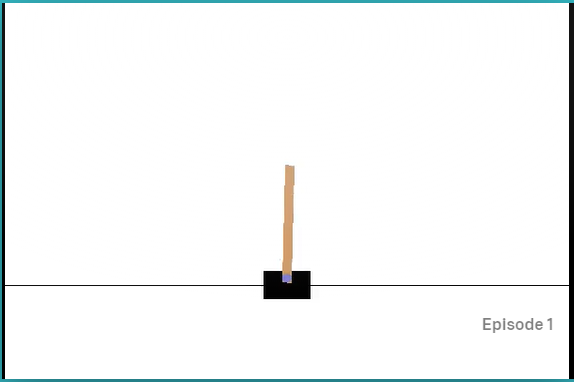
\includegraphics[height=6cm]{images/cartpole.PNG}
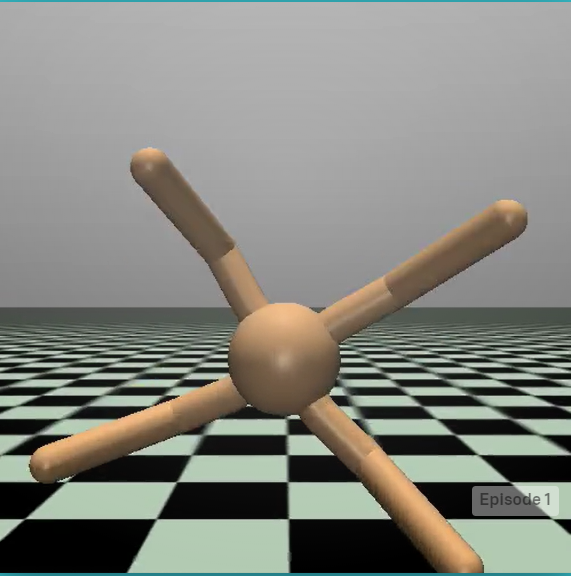
\includegraphics[height=6cm]{images/ant.PNG}
\caption{Cartpole (left) and Ant (right) environments in Gym}
 \small\textsuperscript{\url{https://gym.openai.com/envs/CartPole-v1/} and  \url{http://gym.openai.com/envs/Ant-v2/}}
 \label{fig:gym}
\end{figure}

\subsection{Atari RAM}
% DGW: what is RAM?
Through Gym and the Arcade Learning Environment (ALE, \cite{Atari}), RL algorithms can be trained to play \addlink{https://gym.openai.com/envs/#atari}{Atari games}. While many state-of-the-art reinforcement learning focus on frame-based interaction with the game, requiring GPU computation to process the images through convolutional network, the Atari environments based on RAM (Random-access memory) have been chosen for \berl to reduce training costs and length while still providing complex learning environments. RAM stores all elements and variables of the environment, without introducing the complexity of image-based machine learning. Algorithms benchmarked through \berl hence have to focus more on gameplay than on image processing. 

\section{Algorithms in \berl}

\berl aims at regrouping all state-of-the-art evolutionary RL algorithms in order to compare them. As such, the list of modules we wish to benchmark is still to be completed, but CGP, NEAT and HyperNEAT have already been added. Future development will include Artificial Gene Regulatory Networks \cite{GRN}, Tangled Program Graphs \cite{tpg} and Grammatical Evolution \cite{grammatical-evo}.

\subsection{CGP}

The first algorithm added into \berl is Cartesian Genetic Programming, which was proven efficient on Atari game-playing \cite{CGP}. The \addlink{https://github.com/d9w/CartesianGeneticProgramming.jl}{Julia implementation} used is based on \code{Cambrian.jl} and was developed by Dennis Wilson. The run parameters are based on the CGP parameters used on similar problems. 

\subsection{Neuroevolution algorithms}

As there was no neuroevolution library in Julia to fit the purposes of \berl, I developped \addlink{https://github.com/TemplierPaul/NeuroEvolution.jl}{\neuroevo} to implement NEAT and HyperNEAT.

This library also lays the foundation for the development of more customized neuroevolution algorithms during the second part of my internship, by providing a modular platform based on Cambrian with multiple independent blocks. 

The working principles of NeuroEvolution.jl are detailed in chapter \ref{chap:neuroevo}.

%%% Local Variables: 
%%% mode: latex
%%% TeX-master: "isae-report-template"
%%% End: 